%%%%%%%%%%%%%%%%%%%%%%%%%%%%%%%%%%%%%%%%%
% Stylish Article
% LaTeX Template
% Version 2.1 (1/10/15)
%
% This template has been downloaded from:
% http://www.LaTeXTemplates.com
%
% Original author:
% Mathias Legrand (legrand.mathias@gmail.com) 
% With extensive modifications by:
% Vel (vel@latextemplates.com)
%
% License:
% CC BY-NC-SA 3.0 (http://creativecommons.org/licenses/by-nc-sa/3.0/)
%
%%%%%%%%%%%%%%%%%%%%%%%%%%%%%%%%%%%%%%%%%

%----------------------------------------------------------------------------------------
%	PACKAGES AND OTHER DOCUMENT CONFIGURATIONS
%----------------------------------------------------------------------------------------

\documentclass[fleqn,10pt]{SelfArx} % Document font size and equations flushed left

\usepackage[catalan]{babel} % Specify a different language here - english by default

\usepackage{lipsum} % Required to insert dummy text. To be removed otherwise

%----------------------------------------------------------------------------------------
%	COLUMNS
%----------------------------------------------------------------------------------------

\setlength{\columnsep}{0.55cm} % Distance between the two columns of text
\setlength{\fboxrule}{0.75pt} % Width of the border around the abstract

%----------------------------------------------------------------------------------------
%	COLORS
%----------------------------------------------------------------------------------------

\definecolor{color1}{RGB}{0,0,90} % Color of the article title and sections
\definecolor{color2}{RGB}{0,20,20} % Color of the boxes behind the abstract and headings

%----------------------------------------------------------------------------------------
%	HYPERLINKS
%----------------------------------------------------------------------------------------

\usepackage{hyperref} % Required for hyperlinks
\hypersetup{hidelinks,colorlinks,breaklinks=true,urlcolor=color2,citecolor=color1,linkcolor=color1,bookmarksopen=false,pdftitle={Title},pdfauthor={Author}}

%----------------------------------------------------------------------------------------
%	ARTICLE INFORMATION
%----------------------------------------------------------------------------------------

\JournalInfo{LSMaker: Seminari I} % Journal information
\Archive{Sensor Infrarojos} % Additional notes (e.g. copyright, DOI, review/research article)

\PaperTitle{Sensor Infrarojos} % Article title

\Authors{Nivell de Dificultat: Principiant} % Authors
\affiliation{alloveras@salleurl.edu} % Author affiliation
\affiliation{Departament d'Enginyeria, La Salle Barcelona} % Author affiliation
\Keywords{} % Keywords - if you don't want any simply remove all the text between the curly brackets
\newcommand{\keywordname}{Keywords} % Defines the keywords heading name

%----------------------------------------------------------------------------------------
%	ABSTRACT
%----------------------------------------------------------------------------------------

\Abstract{En aquest seminari es tractarà la implementació d’un sensor que permeti al LSMaker detectar els obstacles del seu entorn.\\

El material necessari és:\\
\begin{itemize}
	\item Ordinador amb MPLAB X i compilador XC-16.
	\item Software Base LSMaker.
	\item Robot LSMaker.
	\item 2 LEDs infrarojos.
	\item 1 Fotodíode receptor d'infrarojos.
\end{itemize}
}

%----------------------------------------------------------------------------------------

\begin{document}

\flushbottom % Makes all text pages the same height

\maketitle % Print the title and abstract box

\tableofcontents % Print the contents section

\thispagestyle{empty} % Removes page numbering from the first page

%----------------------------------------------------------------------------------------
%	ARTICLE CONTENTS
%----------------------------------------------------------------------------------------

\section{Funcionament}

\subsection{Sensor}
Per tal d’explicar la base teòrica del sensor d’infrarrojos
que ens disposem a implementar, us adjuntem les següents il·lustracions:\\

\begin{center}
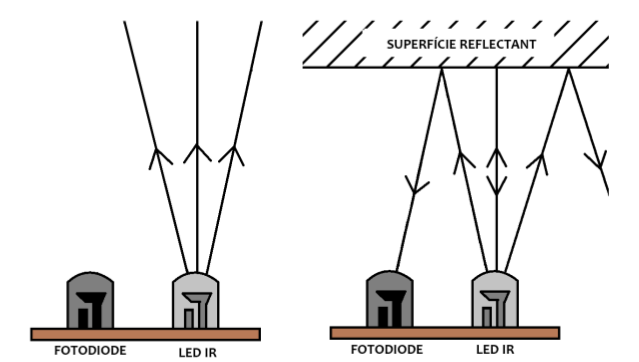
\includegraphics[scale=0.23]{img/img_funcionament_sensor.png}
\end{center}


La il·lustració de l’esquerra mostra com un dels 4 LEDs in-
frarojos del nostre sensor està emetent un feix de llum cap a
l’exterior i, al no trobar cap obstacle al seu davant, aquest feix no es reflectit cap al fotodíode.\\

Contràriament, la il·lustració de la dreta mostra com, en cas
de trobar un obstacle, el fotodíode rep part del feix de llum
infraroja emesa pel LED.
Aquesta configuració de LEDs + Fotodíode ens permet, mitjançant
l’ús d’un petit circuit elèctric, detectar si tenim un obstacle
davant del sensor o no.
A continuació, es proporciona l’esquema elèctric emprat per
a la detecció de presencia juntament amb la seva explicació:
\begin{center}
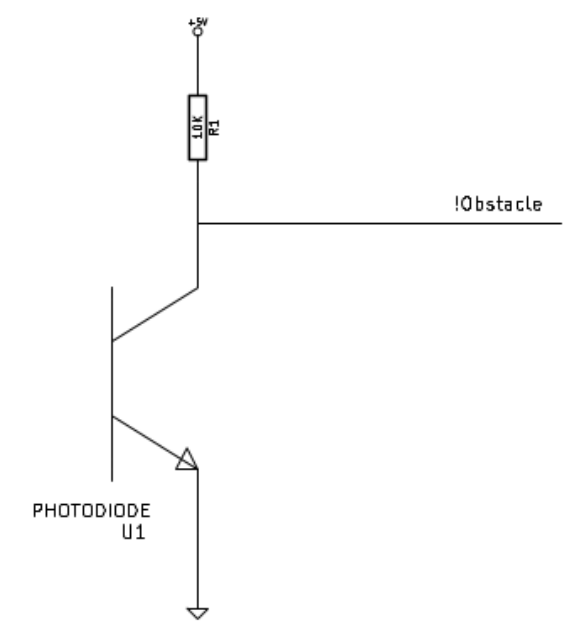
\includegraphics[scale=0.3]{img/img_esquematic.png}
\end{center}

En l’esquemàtic anterior, veiem que el fotodíode està col·locat
en sèrie amb una resistència de 10K. Aquesta configuració
permet el següent:

\begin{itemize}

	\item Quan el fotodíode està tallat: El corrent que passa des del col·lector d'aquest fins al seu emissor és de 0 amperes i, per tant, la tensió entre GND i l’entrada del col·lector és de 5V.

	\item Quan el fotodíode està saturat: El corrent que circula des del col·lector d'aquest fins al seu emissor és superior a 0 amperes i, per tant, la resistència de 10K actua com a divisor de tensió juntament amb el fotodíode

\end{itemize}

D’aquesta manera, podem afirmar que, al punt de mesura del senyal \textit{!Obstacle} la tensió serà bastant inferior a 5 volts. Això es deu a que el corrent col·lector-emissor depèn de la quantitat de llum infraroja incident al fotodíode.\\

Això implica que, contra més llum, més gran
serà el corrent i, per tant, més baixa serà la tensió del senyal \textit{!Obstacle}.


%------------------------------------------------

\section{Detecció via Software}
Un cop explicat com funciona el hardware del sensor d'infrarojos, és el moment d'introduir-nos al processat del senyal \textit{!Obstacle} per mitjà de software.\\

Bàsicament, si ens fixem en l'esquemàtic anterior, veurem que la tensió al punt de mesurà valdrà 5 volts o inferior depenent de si hi ha o no obstacles davant del sensor respectivament. Sabent això, podem plantejar-nos llegir aquest senyal mitjançant un dels pins analògics de l'LSMaker.\\

D'aquesta manera, si mostregem el senyal i el convertim a digital obtindrem una funció semblant a la següent recta:

\begin{center}
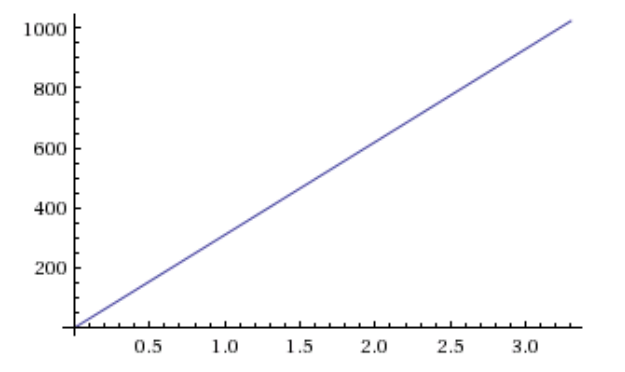
\includegraphics[scale=0.4]{img/img_analog_to_digital.png}
\end{center}

Si ens hi fixem en la gràfica, veurem que, podem relacionar els valors de tensió analògics (eix X) amb un valor decimal de 0 a 1023 (eix Y - resolució de 10 bits). D’aquesta manera, podem realitzar la següent comprovació:

\begin{itemize}

	\item Si valor >= 1000 la tensió està per sobre de 3,2 volts i, llavors, no hi ha obstacle.

	\item Si valor < 1000 la tensió està per sota de 3,2 volts i, llavors, hi ha obstacle.

\end{itemize}


\newpage
Per tal d'obtenir el valor del pin analògic de l'LSMaker que haguem triat farem la següent crida:

\begin{verbatim}
    LS_IO_GetAnalogFiltered(AN_0);
\end{verbatim}

\textbf{Nota:} Cal notar que en el codi anterior, s’ha utilitzat el pin
AN 0 del robot. No obstant, si fos necessari, es podria canviar
per qualsevol dels altres ports analògics i llavors s'hauria d'usar la constant AN\_X de la API que correspongués amb el pin escollit.

\section{Pseudo-codi algorisme}
\begin{verbatim}
1. Comprovar si hi ha un obstacle davant.
Si n’hi ha un, anar al pas 2, sinó avançar
endavant durant 800 milisegons i tornar al
pas 1.

2. Fer un gir de 30 graus a l’esquerra i
mirar si es detecta encara l’obstacle. En
cas afirmatiu, anar al pas 3, sinó avançar
endavant 800 milisegons i tornar al pas 1.

3.Fer un gir de 60 graus a la dreta i
mirar si es detecta encara l’obstacle.
En cas afirmatiu, anar al pas 4. Altrament,
avançar endavant 800 milisegons i tornar
al pas 1.

4. Fer un gir de 150 graus per acabar
de donar la volta completa. Avançar endavant
durant 800 milisegons i tornar al pas 1.
\end{verbatim}

\section{Esquemàtic i Codi}
Aquest document, el codi del seminari i els exemples els podeu trobar al següent enllaç:\\

\small{\url{https://github.com/lsmaker/Seminaris2016}}

%----------------------------------------------------------------------------------------

\end{document}